
% Use only LaTeX2e, calling the article.cls class and 12-point type.
%Tandy is editing on March 6
\documentclass[12pt]{article}

% Users of the {thebibliography} environment or BibTeX should use the
% scicite.sty pack$output_dir/upp_results/upp_$query_size\_$align_size\_mafft_L-INS-i_alignment_masked $output_dir/upp_results/upp_$query_size\_$align_size\_mafft_L-INS-i_alignment_masked age, downloadable from *Science* at
% www.sciencemag.org/about/authors/prep/TeX_help/ .
% This package should properly format in-text
% reference calls and reference-list numbers.  

\usepackage{amsmath}
\usepackage{graphicx}
\usepackage{bigstrut}
\usepackage{color}
\usepackage{multirow}
\usepackage{hhline}
\usepackage{graphics}
\usepackage{hyperref}
\usepackage[export]{adjustbox}
\usepackage{float}
\usepackage{subfig}

% Use times if you have the font installed; otherwise, comment out the
% following line.

\usepackage{times}

% The preamble here sets up a lot of new/revised commands and
% environments.  It's annoying, but please do *not* try to strip these
% out into a separate .sty file (which could lead to the loss of some
% information when we convert the file to other formats).  Instead, keep
% them in the preamble of your main LaTeX source file.

%\externaldocument{hippi_bmc}
% The following parameters seem to provide a reasonable page setup.
\DeclareGraphicsRule{.tif}{png}{.png}{`convert #1 `dirname #1`/`basename #1 .tif`.png}
\topmargin 0.0cm
\oddsidemargin 0.2cm
\textwidth 16cm 
\textheight 21cm
\footskip 1.0cm


%\renewcommand\refname{References and Notes}

% The following lines set up an environment for the last note in the
% reference list, which commonly includes acknowledgments of funding,
% help, etc.  It's intended for users of BibTeX or the {thebibliography}
% environment.  Users who are hand-coding their references at the end
% using a list environment such as {enumerate} can simply add another
% item at the end, and it will be numbered automatically.

\newcounter{lastnote}
\newenvironment{scilastnote}{%
\setcounter{lastnote}{\value{enumiv}}%
\addtocounter{lastnote}{+1}%
\begin{list}%
{\arabic{lastnote}.}
{\setlength{\leftmargin}{.22in}}
{\setlength{\labelsep}{.5em}}}
{\end{list}}


% Include your paper's title here

\title{ViFi Supplement} 


% Place the author information here.  Please hand-code the contact
% information and notecalls; do *not* use \footnote commands.  Let the
% author contact information appear immediately below the author names
% as shown.  We would also prefer that you don't change the type-size
% settings shown here.

\author
{Nam-phuong Nguyen$^{1}$, Viraj Deshpande$^{1}$, Jens Luebeck$^{1}$, and Vineet Bafna$^{1\ast}$\\
\\
\normalsize{$^{1}$Computer Science and Engineering, University of California, San Diego,}\\
\normalsize{$^\ast$To whom correspondence should be addressed; E-mail: vbafna@cs.ucsd.edu.}
}

\appendix
\setcounter{figure}{0}
\renewcommand{\thesection}{S.\arabic{section}}   
\renewcommand{\thefigure}{S\arabic{figure}}   
\renewcommand{\thetable}{S\arabic{table}}   

%%%%%%%%%%%%%%%%% END OF PREAMBLE %%%%%%%%%%%%%%%%



\begin{document} 
\sloppy
% Double-space the manuscript.

\baselineskip24pt

% Make the title.

\maketitle 

% In setting up this template for *Science* papers, we've used both
% the \section* command and the \paragraph* command for topical
% divisions.  Which you use will of course depend on the type of paper
% you're writing.  Review Articles tend to have displayed headings, for
% which \section* is more appropriate; Research Articles, when they have
% formal topical divisions at all, tend to signal them with bold text
% that runs into the paragraph, for which \paragraph* is the right
% choice.  Either way, use the asterisk (*) modifier, as shown, to
% suppress numbering.


\tableofcontents
\clearpage
\listoffigures
\clearpage
\listoftables
\clearpage


\begin{figure}[htpb]
  \centering
  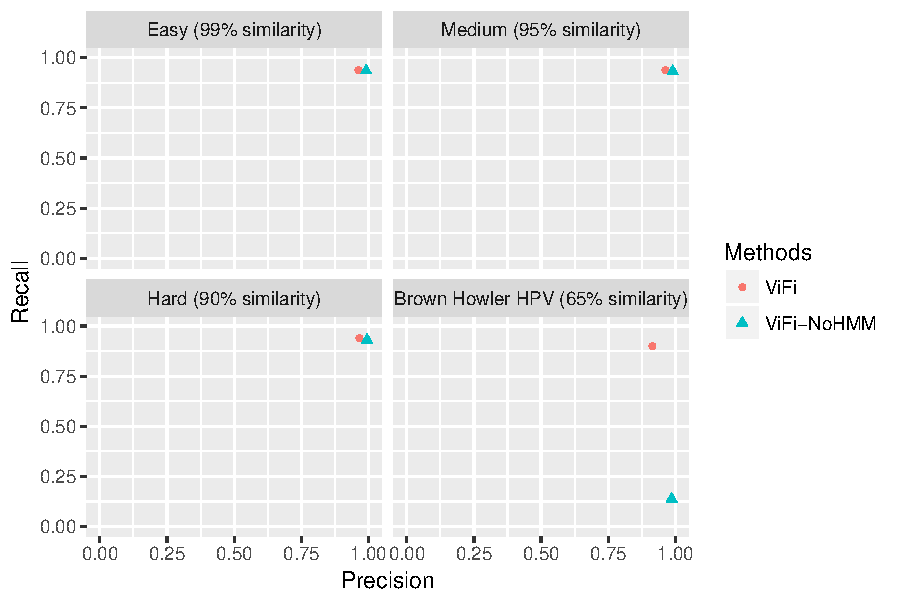
\includegraphics[width=1\linewidth]{{results/simulation.1000}.pdf}\\
  \caption[Precision-recall on simulated datasets with 1000 viral integrations.] {{\bf Precision-recall on simulated datasets.  \label{sim_results_1000}}  We report the recall and precision for four different model conditions.  We show results for when we include the usage of the  ensemble of HMMs in detecting viral reads (Default) and when we exclude the usage of the ensemble of HMMs (Default-NoHMMs).  The first three model conditions (easy, medium, and hard) vary the percent similarity of simulated HPV16 genomes to the reference HPV16 genome, with five replicates per simulation.  The last model condition uses Alouatta guariba papillomavirus 1 (AgPV1), an HPV genome not included in the set of viral genomes to simulate detection of a novel HPV virus.  AgPV1 is 44\% similar to HPV16.  VERSE failed complete on any datasets.  All datasets were simulated with 25x coverage.}
\end{figure}

\begin{figure}[htpb]
  \centering
  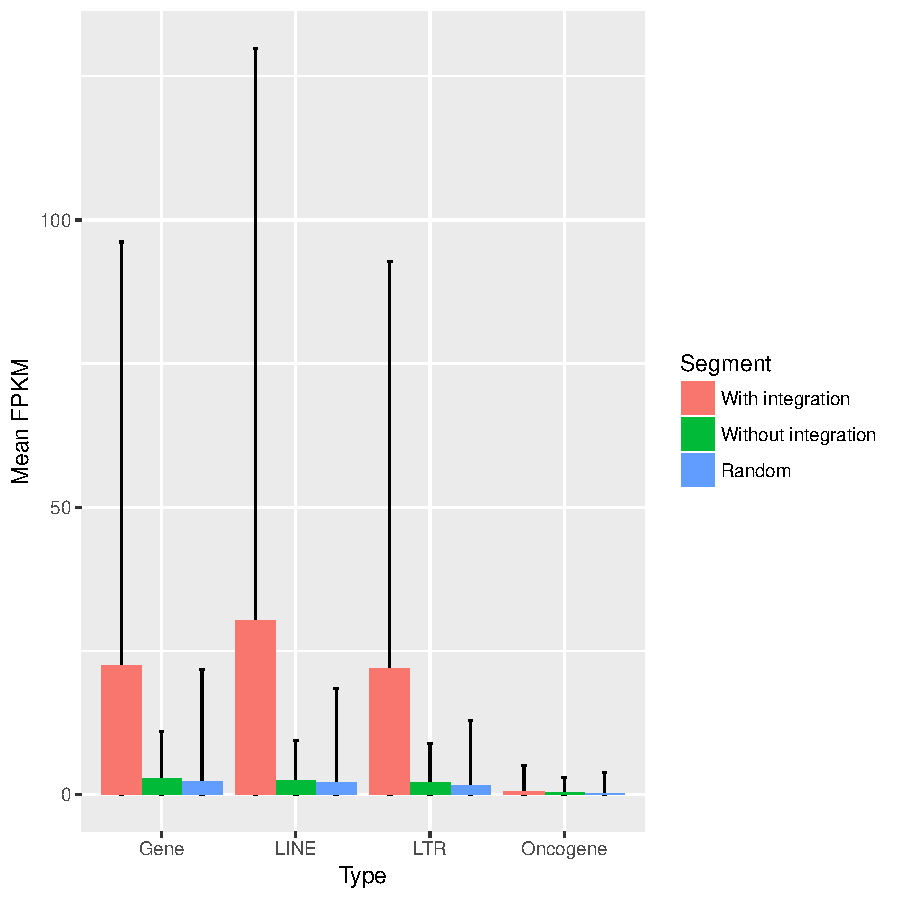
\includegraphics[width=1\linewidth]{{results/expression.summary.barplot}.pdf}\\
\caption[Expression of mRNA transcripts in genomic segments with and without integrations.]
{\label{expression_transcripts_fpkm}  {\bf Expression of mRNA transcripts in genomic segments with and without integrations.}  We report the mean FPKM expression of annotated features in genomic segments with and without integrations.  For a given integration in a sample, we select a 10kb flanking region around the integration site.  We then report the expression level in samples that have an integration in this region and samples that do not.  In addition, we report the expression level randomly selected segments as a baseline. The p-values for the paired Wilcoxon signed rank test of the difference in FPKM expression for genomic segments with and mean FPKM expression in segments without integrations are: LINE < 1e-12;	LTR < 1e-10;  Gene < 1e-10; and	Oncogenes < NA.}
\end{figure}



\begin{figure}[htpb]
  \centering
  
\includegraphics[width=0.75\linewidth]{{results/fusion_TCGA-C5-A0TN}.pdf}\\
  \caption[Example of fusion mRNA found by ViFi.] {{\bf Example of fusion mRNA found by ViFi  \label{vifi_exmaple}}  We show an example of a fusion mRNA event found by ViFi that was not reported by the Tang et al. 2014 study nor found by VERSE for the sample TCGA-C5-A0TN on the genomic segment chr3:126,847,238-126,849,346.  The first track is the results from mapping the RNA-seq data, and the second track is the results from mapping the WGS data.  Reads in red are chimeric reads in which one end maps to the human hg19 reference (shown) and the other end maps to the viral reference.  The results show that both the top and bottom track contain chimeric reads clustered around this interval.}
\end{figure}


\begin{figure}[htpb]
  \centering
  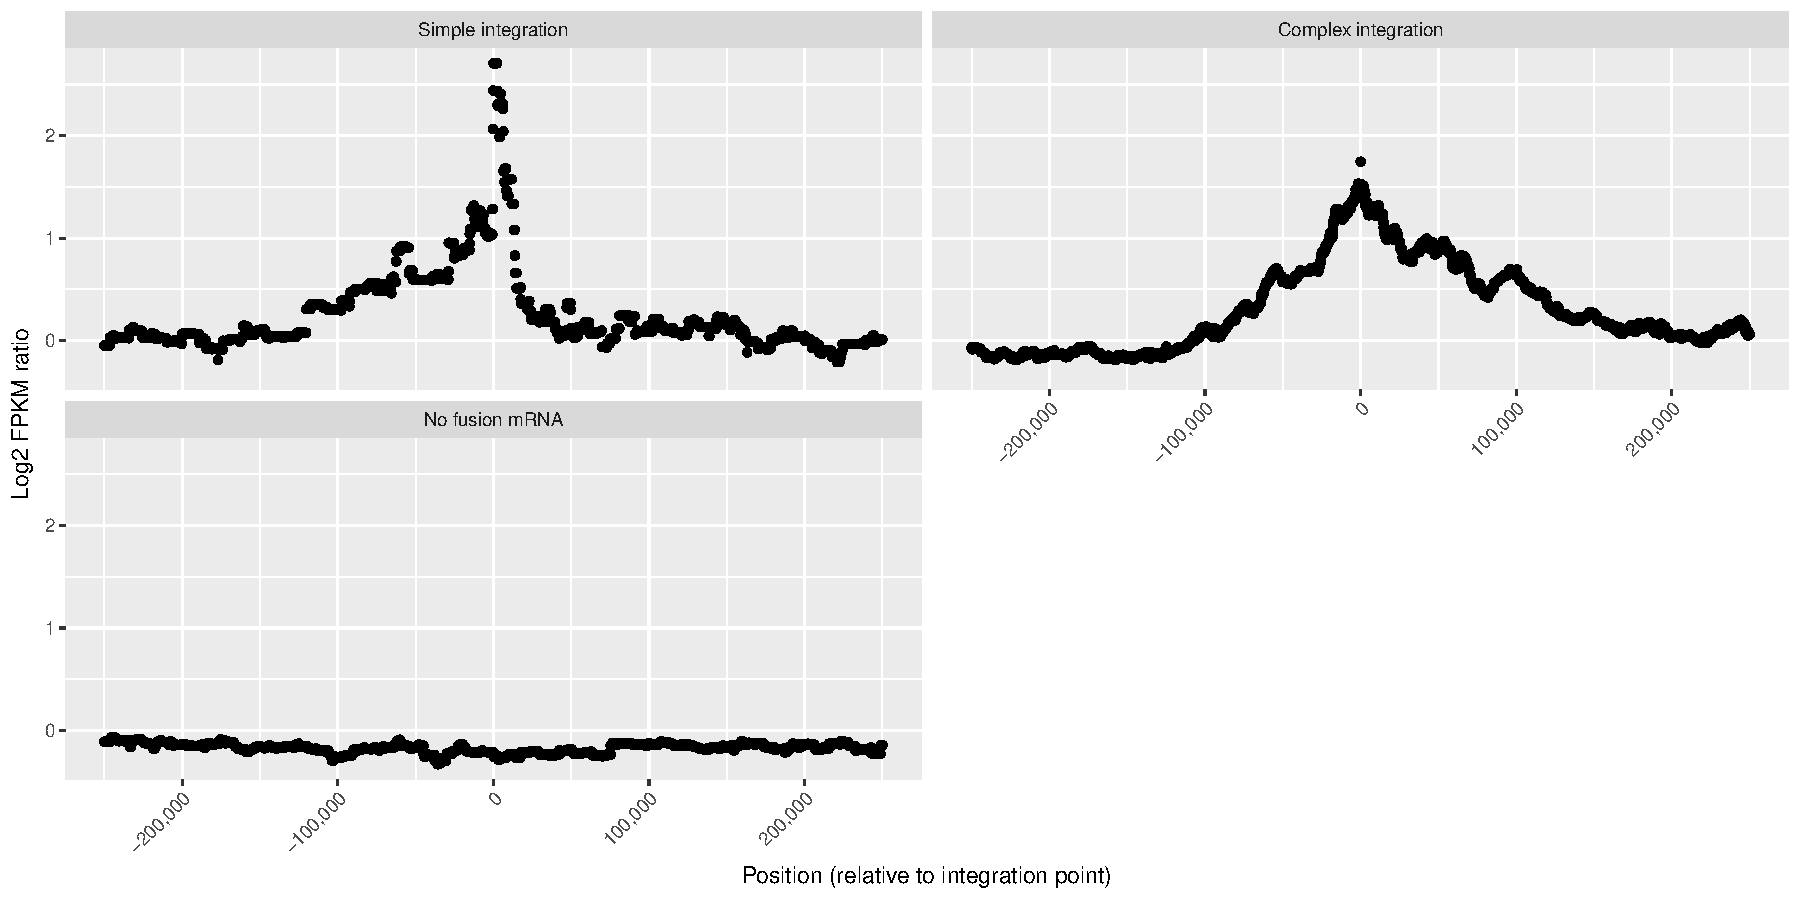
\includegraphics[width= 4in,frame]{{results/updown.250000}.pdf}
\caption[Fusion reads supp.]
{\label{updown}  {\bf Expression change around integration point within a 250kb window}.  We report the average log-fold expression change upstream and downstream of an integration event within a 250kb window.  The position is reported relative to the integration point in the human genome, with negative position being upstream of the integration event, and positive position being downstream of the integration event.  The results are separated out by the integration category. } %35, 110, 81
\end{figure}
\clearpage
\bibliographystyle{natbib}
\bibliography{main}
\end{document}
